\chapter{Ahneet algoritmit}

\index{ahne algoritmi}

\key{Ahne algoritmi}
muodostaa ongelman ratkaisun
tekemällä joka askeleella
sillä hetkellä parhaalta näyttävän valinnan.
Ahne algoritmi ei koskaan 
peruuta tekemiään valintoja vaan
muodostaa ratkaisun suoraan valmiiksi.
Tämän ansiosta ahneet algoritmit ovat
yleensä hyvin tehokkaita.

Vaikeutena ahneissa algoritmeissa on
keksiä toimiva ahne strategia,
joka tuottaa aina optimaalisen ratkaisun tehtävään.
Ahneen algoritmin tulee olla sellainen,
että kulloinkin parhaalta näyttävät valinnat
tuottavat myös parhaan kokonaisuuden.
Tämän perusteleminen on usein hankalaa.

\section{Kolikkotehtävä}

Aloitamme ahneisiin algoritmeihin tutustumisen
seuraavasta tehtävästä:

\begin{task}
Kolikoiden arvot ovat $\{c_1,c_2,\ldots,c_k\}$,
ja tehtäväsi on muodostaa kolikoista rahamäärä $x$.
Jokaista kolikkoa on saatavilla rajattomasti.
Mikä on pienin määrä kolikoita,
joilla rahamäärän voi muodostaa?
\end{task}

\noindent
Esimerkiksi jos kolikot ovat eurokolikot eli sentteinä
\[\{1,2,5,10,20,50,100,200\}\]
ja muodostettava rahamäärä on 520,
kolikoita tarvitaan vähintään 4.
Optimiratkaisu on valita kolikot $200+200+100+20$.

\subsubsection{Ahne algoritmi}

Luonteva ahne algoritmi tehtävään
on poistaa rahamäärästä aina mahdollisimman
suuri kolikko, kunnes rahamäärä on 0.
Tämä algoritmi toimii esimerkissä,
koska rahamäärästä 520 
poistetaan ensin kahdesti 200, sitten 100
ja lopuksi 20.
Mutta toimiiko ahne algoritmi aina oikein?

Osoittautuu, että eurokolikoiden tapauksessa
ahne algoritmi toimii aina oikein,
eli se tuottaa aina ratkaisun,
jossa on pienin määrä kolikoita.
Algoritmin toimivuuden voi perustella
seuraavasti:

Kutakin kolikkoa 1, 5, 10, 50 ja 100
on optimiratkaisussa enintään yksi.
Tämä johtuu siitä, että jos
ratkaisussa olisi kaksi tällaista kolikkoa,
saman ratkaisun voisi muodostaa
käyttäen vähemmän kolikoita.
Esimerkiksi jos ratkaisussa on
kolikot $5+5$, ne voi korvata kolikolla 10.

Vastaavasti kumpaakin kolikkoa 2 ja 20
on optimiratkaisussa enintään kaksi,
koska kolikot $2+2+2$ voi korvata kolikoilla $1+5$
ja kolikot $20+20+20$ voi korvata kolikoilla $10+50$.
Lisäksi ratkaisussa ei voi olla yhdistelmiä
$1+2+2$ ja $10+20+20$,
koska ne voi korvata kolikoilla 5 ja 50.

Näiden havaintojen perusteella
jokaiselle kolikolle $x$ pätee,
että $x$:ää pienemmistä kolikoista
ei ole mahdollista saada aikaan summaa
$x$ tai suurempaa summaa optimaalisesti.
Esimerkiksi jos $x=100$, pienemmistä kolikoista
saa korkeintaan summan $50+20+20+5+2+2=99$.
Niinpä ahne algoritmi,
joka valitsee aina suurimman kolikon,
tuottaa optimiratkaisun.

Kuten tästä esimerkistä huomaa,
ahneen algoritmin toimivuuden perusteleminen
voi olla vaikeaa,
vaikka kyseessä olisi yksinkertainen algoritmi.

\subsubsection{Yleinen tapaus}

Yleisessä tapauksessa kolikot voivat olla mitä tahansa.
Tällöin suurimman kolikon valitseva ahne algoritmi
ei välttämättä tuota optimiratkaisua.

Jos ahne algoritmi ei toimi, tämän voi osoittaa
näyttämällä vastaesimerkin, jossa algoritmi
antaa väärän vastauksen.
Tässä tehtävässä vastaesimerkki on helppoa keksiä:
jos kolikot ovat $\{1,3,4\}$ ja muodostettava
rahamäärä on 6, ahne algoritmi tuottaa ratkaisun
$1+1+4$, kun taas optimiratkaisu on $3+3$.

Yleisessä tapauksessa tehtävän ratkaisuun
ei tunneta ahnetta algoritmia,
mutta palaamme tehtävään seuraavassa luvussa.
Tehtävään on nimittäin olemassa dynaamista
ohjelmointia käyttävä algoritmi,
joka tuottaa optimiratkaisun
millä tahansa kolikoilla ja rahamäärällä.

\section{Aikataulutus}

Monet aikataulutukseen liittyvät ongelmat
ratkeavat ahneasti.
Näin on esimerkiksi seuraavassa klassisessa tehtävässä:

\begin{task}
Annettuna on $n$ tapahtumaa,
jotka alkavat ja päättyvät tiettyinä hetkinä.
Tehtäväsi on suunnitella aikataulu,
jota seuraamalla pystyt osallistumaan
mahdollisimman moneen tapahtumaan.
Et voi osallistua tapahtumaan vain osittain.
\end{task}

Esimerkiksi jos tapahtumat ovat

\begin{center}
\begin{tabular}{lll}
tapahtuma & alkuaika & loppuaika \\
\hline
$A$ & 1 & 3 \\
$B$ & 2 & 5 \\
$C$ & 3 & 9 \\
$D$ & 6 & 8 \\
\end{tabular}
\end{center}

\noindent
niin on mahdollista osallistua korkeintaan
kahteen tapahtumaan.
Yksi mahdollisuus on osallistua tapahtumiin
$B$ ja $D$ seuraavasti:
\\
\begin{center}
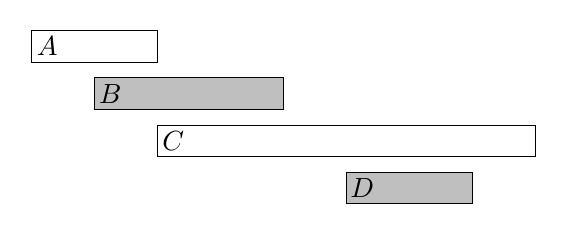
\begin{tikzpicture}[scale=.4]
  \begin{scope}
    \draw (2, 0) rectangle (6, -1);
    \draw[fill=lightgray] (4, -1.5) rectangle (10, -2.5);
    \draw (6, -3) rectangle (18, -4);
    \draw[fill=lightgray] (12, -4.5) rectangle (16, -5.5);
    \node at (2.5,-0.5) {$A$};
    \node at (4.5,-2) {$B$};
    \node at (6.5,-3.5) {$C$};
    \node at (12.5,-5) {$D$};
  \end{scope}
\end{tikzpicture}
\end{center}

\noindent
Tehtävän ratkaisuun on mahdollista 
keksiä useita ahneita algoritmeja,
mutta mikä niistä toimii kaikissa tapauksissa?

\subsubsection*{Algoritmi 1}

Ensimmäinen idea on valita ratkaisuun
mahdollisimman lyhyitä tapahtumia.
Esimerkin tapauksessa tällainen
algoritmi valitsee tapahtumat
\\
\begin{center}
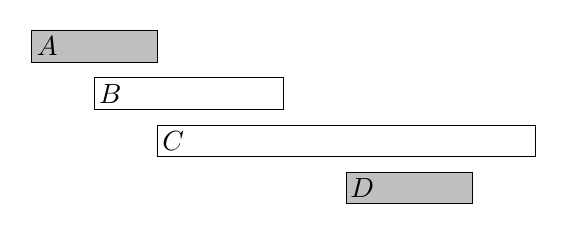
\begin{tikzpicture}[scale=.4]
  \begin{scope}
    \draw[fill=lightgray] (2, 0) rectangle (6, -1);
    \draw (4, -1.5) rectangle (10, -2.5);
    \draw (6, -3) rectangle (18, -4);
    \draw[fill=lightgray] (12, -4.5) rectangle (16, -5.5);
    \node at (2.5,-0.5) {$A$};
    \node at (4.5,-2) {$B$};
    \node at (6.5,-3.5) {$C$};
    \node at (12.5,-5) {$D$};
  \end{scope}
\end{tikzpicture}
\end{center}
ja tuottaa optimiratkaisun.

Lyhimpien tapahtumien valinta ei ole kuitenkaan
aina toimiva strategia.
Algoritmi epäonnistuu esimerkiksi seuraavassa tilanteessa:
\\
\begin{center}
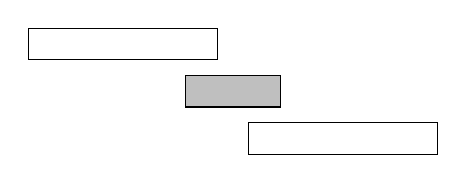
\begin{tikzpicture}[scale=.4]
  \begin{scope}
    \draw (1, 0) rectangle (7, -1);
    \draw[fill=lightgray] (6, -1.5) rectangle (9, -2.5);
    \draw (8, -3) rectangle (14, -4);
  \end{scope}
\end{tikzpicture}
\end{center}

Kun lyhyt tapahtuma valitaan mukaan,
on mahdollista osallistua vain yhteen tapahtumaan.
Kuitenkin valitsemalla pitkät tapahtumat
olisi mahdollista osallistua kahteen tapahtumaan.

\subsubsection*{Algoritmi 2}

Toinen idea on valita aina seuraavaksi tapahtuma,
joka alkaa mahdollisimman aikaisin.
Tämä algoritmi valitsee esimerkissä tapahtumat
\\
\begin{center}
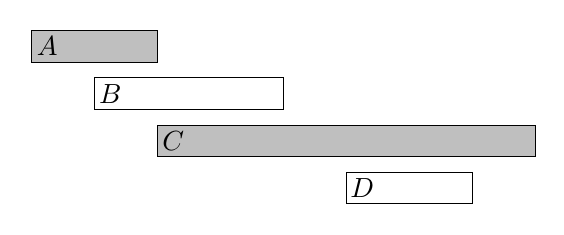
\begin{tikzpicture}[scale=.4]
  \begin{scope}
    \draw[fill=lightgray] (2, 0) rectangle (6, -1);
    \draw (4, -1.5) rectangle (10, -2.5);
    \draw[fill=lightgray] (6, -3) rectangle (18, -4);
    \draw (12, -4.5) rectangle (16, -5.5);
    \node at (2.5,-0.5) {$A$};
    \node at (4.5,-2) {$B$};
    \node at (6.5,-3.5) {$C$};
    \node at (12.5,-5) {$D$};
  \end{scope}
\end{tikzpicture}
\end{center}
ja tuottaa optimiratkaisun.

Tämä algoritmi ei kuitenkaan toimi
esimerkiksi seuraavassa tilanteessa:
\\
\begin{center}
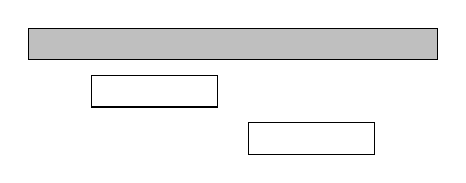
\begin{tikzpicture}[scale=.4]
  \begin{scope}
    \draw[fill=lightgray] (1, 0) rectangle (14, -1);
    \draw (3, -1.5) rectangle (7, -2.5);
    \draw (8, -3) rectangle (12, -4);
  \end{scope}
\end{tikzpicture}
\end{center}

Kun ensimmäisenä alkava tapahtuma
valitaan mukaan, mitään muuta tapahtumaa
ei ole mahdollista valita.
Kuitenkin olisi mahdollista osallistua
kahteen tapahtumaan valitsemalla
kaksi myöhempää tapahtumaa.

\subsubsection*{Algoritmi 3}

Kolmas idea on valita aina seuraavaksi tapahtuma,
joka päättyy mahdollisimman aikaisin.
Tämä algoritmi valitsee esimerkissä tapahtumat
\\
\begin{center}
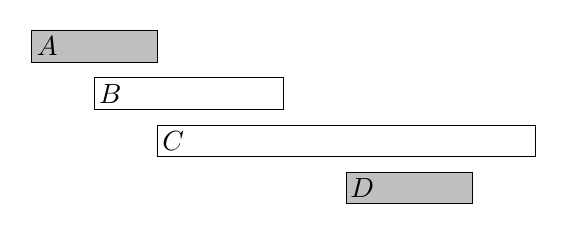
\begin{tikzpicture}[scale=.4]
  \begin{scope}
    \draw[fill=lightgray] (2, 0) rectangle (6, -1);
    \draw (4, -1.5) rectangle (10, -2.5);
    \draw (6, -3) rectangle (18, -4);
    \draw[fill=lightgray] (12, -4.5) rectangle (16, -5.5);
    \node at (2.5,-0.5) {$A$};
    \node at (4.5,-2) {$B$};
    \node at (6.5,-3.5) {$C$};
    \node at (12.5,-5) {$D$};
  \end{scope}
\end{tikzpicture}
\end{center}
ja tuottaa optimiratkaisun.

Osoittautuu, että tämä ahne algoritmi
tuottaa \textit{aina} optimiratkaisun.
Algoritmi toimii, koska on aina kokonaisuuden
kannalta optimaalista valita
ensimmäiseksi tapahtumaksi
mahdollisimman aikaisin päättyvä tapahtuma.
Tämän jälkeen on taas optimaalista
valita seuraava aikatauluun sopiva
mahdollisimman aikaisin
päättyvä tapahtua, jne.

Yksi tapa perustella valintaa on miettiä,
mitä tapahtuu, jos ensimmäiseksi tapahtumaksi
valitaan jokin muu kuin mahdollisimman
aikaisin päättyvä tapahtuma.
Tällainen valinta ei ole koskaan parempi,
koska myöhemmin päättyvän tapahtuman
jälkeen on joko yhtä paljon tai vähemmän
mahdollisuuksia valita seuraavia tapahtumia.

\section{Tehtävät ja deadlinet}

\begin{task}
Annettuna on $n$ tehtävää,
joista jokaisella on kesto ja deadline.
Tehtäväsi on valita järjestys,
jossa suoritat tehtävät.
Saat kustakin tehtävästä $d-x$ pistettä,
missä $d$ on tehtävän deadline ja $x$
on tehtävän valmistumishetki.
Mikä on suurin mahdollinen pistesumma?
\end{task}

Esimerkiksi jos tehtävät ovat

\begin{center}
\begin{tabular}{lll}
tehtävä & kesto & deadline \\
\hline
$A$ & 4 & 2 \\
$B$ & 3 & 5 \\
$C$ & 2 & 7 \\
$D$ & 4 & 5 \\
\end{tabular}
\end{center}

\noindent
niin optimaalinen ratkaisu on suorittaa
tehtävät seuraavasti:

\begin{center}
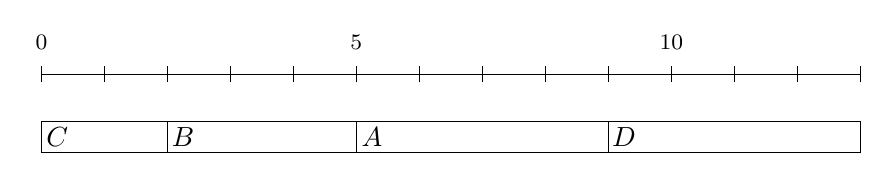
\begin{tikzpicture}[scale=.4]
  \begin{scope}
    \draw (0, 0) rectangle (4, -1);
    \draw (4, 0) rectangle (10, -1);
    \draw (10, 0) rectangle (18, -1);
    \draw (18, 0) rectangle (26, -1);
    \node at (0.5,-0.5) {$C$};
    \node at (4.5,-0.5) {$B$};
    \node at (10.5,-0.5) {$A$};
    \node at (18.5,-0.5) {$D$};

    \draw (0,1.5) -- (26,1.5);
    \foreach \i in {0,2,...,26}
    {
        \draw (\i,1.25) -- (\i,1.75);
    }
    \footnotesize
    \node at (0,2.5) {0};
    \node at (10,2.5) {5};
    \node at (20,2.5) {10};

  \end{scope}
\end{tikzpicture}
\end{center}

Tässä ratkaisussa $C$ tuottaa 5 pistettä,
$B$ tuottaa 0 pistettä, $A$ tuottaa $-7$ pistettä
ja $D$ tuottaa $-8$ pistettä,
joten pistesumma on $-10$.

Yllättävää kyllä, tehtävän optimaalinen ratkaisu
ei riipu lainkaan deadlineista.
Toimiva ahne strategia on
suorittaa tehtävät järjestyksessä keston mukaan
lyhimmästä pisimpään.
Syynä tähän on, että jos missä tahansa vaiheessa
suoritetaan peräkkäin kaksi tehtävää,
joista ensimmäinen kestää toista kauemmin,
tehtävien järjestyksen vaihtaminen parantaa ratkaisua.

Esimerkiksi jos peräkkäin ovat tehtävät

\begin{center}
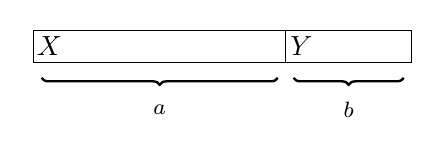
\begin{tikzpicture}[scale=.4]
  \begin{scope}
    \draw (0, 0) rectangle (8, -1);
    \draw (8, 0) rectangle (12, -1);
    \node at (0.5,-0.5) {$X$};
    \node at (8.5,-0.5) {$Y$};

\draw [decoration={brace}, decorate, line width=0.3mm] (7.75,-1.5) -- (0.25,-1.5);
\draw [decoration={brace}, decorate, line width=0.3mm] (11.75,-1.5) -- (8.25,-1.5);

\footnotesize
\node at (4,-2.5) {$a$};
\node at (10,-2.5) {$b$};

  \end{scope}
\end{tikzpicture}
\end{center}

ja $a>b$, niin järjestyksen muuttaminen muotoon

\begin{center}
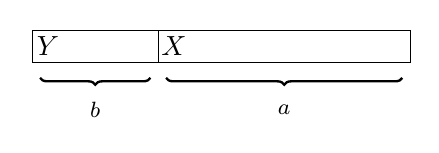
\begin{tikzpicture}[scale=.4]
  \begin{scope}
    \draw (0, 0) rectangle (4, -1);
    \draw (4, 0) rectangle (12, -1);
    \node at (0.5,-0.5) {$Y$};
    \node at (4.5,-0.5) {$X$};

\draw [decoration={brace}, decorate, line width=0.3mm] (3.75,-1.5) -- (0.25,-1.5);
\draw [decoration={brace}, decorate, line width=0.3mm] (11.75,-1.5) -- (4.25,-1.5);

\footnotesize
\node at (2,-2.5) {$b$};
\node at (8,-2.5) {$a$};

  \end{scope}
\end{tikzpicture}
\end{center}

antaa $X$:lle $b$ pistettä vähemmän ja $Y$:lle $a$ pistettä enemmän,
joten kokonaismuutos pistemäärään on $a-b > 0$.
Optimiratkaisussa
kaikille peräkkäin suoritettaville tehtäville
tulee päteä, että lyhyempi tulee ennen pidempää,
mistä seuraa, että tehtävät tulee suorittaa
järjestyksessä keston mukaan.

\section{Keskiluvut}

\subsubsection{Itseisarvosumma}

\begin{task}
Annettuna on $n$ lukua $a_1,a_2,\ldots,a_n$.
Tehtäväsi on etsiä luku $x$, joka minimoi summan
$|a_1-x|+|a_2-x|+\cdots+|a_n-x|.$
\end{task}

Esimerkiksi jos luvut ovat $[1,2,9,2,6]$,
niin paras ratkaisu on $x=2$,
jolloin summaksi tulee
\[
|1-2|+|2-2|+|9-2|+|2-2|+|6-2|=12.
\]

Yleisessä tapauksessa paras valinta $x$:n arvoksi
on lukujen \textit{mediaani}
eli keskimmäinen luku järjestyksessä.
Esimerkiksi luvut $[1,2,9,2,6]$
ovat järjestyksessä $[1,2,2,6,9]$,
joten mediaani on 2.

Mediaanin valinta on paras ratkaisu,
koska jos $x$ on mediaania pienempi,
$x$:n suurentaminen pienentää summaa.
Vastaavasti jos $x$ on mediaania suurempi,
$x$:n pienentäminen pienentää summaa.
Niinpä $x$ kannattaa siirtää mahdollisimman
lähelle mediaania eli optimiratkaisu on
valita $x$ mediaaniksi.

Jos $n$ on parillinen ja mediaaneja on kaksi,
kumpikin mediaani sekä kaikki niiden välillä
olevat luvut tuottavat optimaalisen ratkaisun.

\subsubsection{Neliösumma}

\begin{task}
Annettuna on $n$ lukua $a_1,a_2,\ldots,a_n$.
Tehtäväsi on etsiä luku $x$, joka minimoi summan
$(a_1-x)^2+(a_2-x)^2+\cdots+(a_n-x)^2.$
\end{task}

Esimerkiksi jos luvut ovat $[1,2,9,2,6]$,
niin paras ratkaisu on $x=4$,
jolloin summaksi tulee
\[
(1-4)^2+(2-4)^2+(9-4)^2+(2-4)^2+(6-4)^2=46.
\]

\noindent
Nyt yleisessä tapauksessa
paras valinta $x$:n arvoksi on lukujen
\textit{keskiarvo}.
Esimerkissä lukujen keskiarvo on $(1+2+9+2+6)/5=4$.

Tämän tuloksen voi johtaa järjestämällä summan
uudestaan muotoon

\[
(a_1^2+a_2^2+\cdots+a_n^2)-2x(a_1+a_2+\cdots+a_n)+nx^2.
\]

Ensimmäinen osa ei riipu $x$:stä, joten sen voi jättää huomiotta.
Jäljelle jäävistä osista muodostuu funktio
$nx^2-2xs$, missä $s=a_1+a_2+\cdots+a_n$.
Tämä on ylöspäin aukeava paraabeli,
jonka nollakohdat ovat $x=0$ ja $x=2s/n$
ja pienin arvo on näiden keskikohta
$x=s/n$ eli taulukon lukujen keskiarvo.

\section{Huffmanin koodaus}

\index{Huffmanin koodaus}
\index{koodi}
\index{koodisana}
\index{binäärikoodi}

Tarkastellaan tehtävää, jossa annettuna on merkkijono ja
sille tulee muodostaa \key{koodi},
jossa jokaista merkkiä vastaa tietty \key{koodisana}.
Oletetaan, että koodin tulee olla \key{binäärikoodi}
eli koodisanojen tulee muodostua biteistä 0 ja 1.
Tällaisen koodin avulla voidaan muodostaa merkkijonoa
vastaava bittiesitys.

Yksi mahdollisuus on muodostaa vakiopituinen
koodi eli valita koodisanat niin,
että jokaisen koodisanan pituus on sama.
Esimerkiksi jos aakkostossa on neljä merkkiä,
tarvittava koodisanan pituus on 2:
\begin{center}
\begin{tabular}{rr}
merkki & koodisana \\
\hline
\texttt{A} & 00 \\
\texttt{B} & 01 \\
\texttt{C} & 10 \\
\texttt{D} & 11 \\
\end{tabular}
\end{center}
Nyt esimerkiksi merkkijonoa \texttt{AABACDACA}
vastaa seuraava bittiesitys, jonka pituus on 18 bittiä:
\[000001001011001000\]
Bittiesitystä on kuitenkin mahdollista lyhentää
ottamalla käyttöön koodi, jonka koodisanat voivat
olla keskenään eripituisia.
Ideana on valita usein esiintyville merkeille
lyhyitä koodisanoja ja harvoin esiintyville
merkeille pitkiä koodisanoja.
Tässä tapauksessa hyvä koodi on seuraava:
\begin{center}
\begin{tabular}{rr}
merkki & koodisana \\
\hline
\texttt{A} & 0 \\
\texttt{B} & 110 \\
\texttt{C} & 10 \\
\texttt{D} & 111 \\
\end{tabular}
\end{center}
Nyt merkkijonon \texttt{AABACDACA}
bittiesityksen pituus on vain 15:
\[001100101110100\]
Huomaa, että koodissa ei saa esiintyä kahta koodisanaa,
joista toinen on toisen alkuosa,
koska alkuperäisen merkkijonon palauttaminen
bittiesityksestä ei olisi välttämättä mahdollista.
Esimerkiksi koodissa
\begin{center}
\begin{tabular}{rr}
merkki & koodisana \\
\hline
\texttt{A} & 0 \\
\texttt{B} & 00 \\
\texttt{C} & 1 \\
\texttt{D} & 11 \\
\end{tabular}
\end{center}
koodisan 0 on koodisanan 00 alkuosa.
Tämän seurauksena ei ole mahdollista tietää, tarkoittaako bittiesitys
001 merkkijonoa \texttt{AAC} vai merkkijonoa \texttt{BC}.

\subsubsection{Optimaalinen koodi}

Optimaalinen koodi on sellainen, jossa merkkijonon bittiesitys
on mahdollisimman lyhyt.
Esimerkiksi merkkijonon \texttt{AABACDACA} tapauksessa
optimaalinen koodi on yllä esitetty koodi,
jota käyttäen bittiesityksen pituus on 15.

\key{Huffmanin koodaus} on yleinen menetelmä,
jonka avulla voi muodostaa optimaalisen koodin merkkijonolle.
Siinä on ideana muodostaa koodia vastaava binääripuu
merkkien esiintymiskertojen perusteella.

Aluksi jokaista merkkijonon merkkiä vastaa solmu,
jonka painona on merkin esiintymiskertojen määrä merkkijonossa.
Tämän jälkeen joka vaiheessa yhdistetään kaksi solmua,
joiden painot ovat pienimmät.
Näin jatketaan, kunnes koodi on valmis.

Esimerkiksi merkkijonon \texttt{AABACDACA} tapauksessa
alkutilanne on seuraava:

\begin{center}
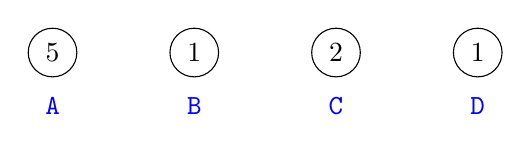
\begin{tikzpicture}[scale=0.9]
\node[draw, circle] (1) at (0,0) {$5$};
\node[draw, circle] (2) at (2,0) {$1$};
\node[draw, circle] (3) at (4,0) {$2$};
\node[draw, circle] (4) at (6,0) {$1$};

\node[color=blue] at (0,-0.75) {\texttt{A}};
\node[color=blue] at (2,-0.75) {\texttt{B}};
\node[color=blue] at (4,-0.75) {\texttt{C}};
\node[color=blue] at (6,-0.75) {\texttt{D}};

%\path[draw,thick,-] (4) -- (5);
\end{tikzpicture}
\end{center}
Merkkiä \texttt{A} vastaavan solmun paino on
5, koska merkki \texttt{A} esiintyy 5 kertaa merkkijonossa.
Muiden solmujen painot on laskettu vastaavalla tavalla.

Ensimmäinen askel on yhdistää merkkejä \texttt{B} ja \texttt{D}
vastaavat solmut, joiden kummankin paino on 1.
Tuloksena on:
\begin{center}
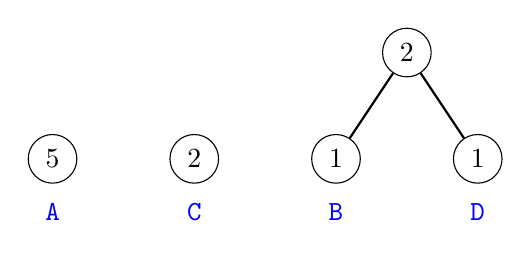
\begin{tikzpicture}[scale=0.9]
\node[draw, circle] (1) at (0,0) {$5$};
\node[draw, circle] (3) at (2,0) {$2$};
\node[draw, circle] (2) at (4,0) {$1$};
\node[draw, circle] (4) at (6,0) {$1$};
\node[draw, circle] (5) at (5,1.5) {$2$};

\node[color=blue] at (0,-0.75) {\texttt{A}};
\node[color=blue] at (2,-0.75) {\texttt{C}};
\node[color=blue] at (4,-0.75) {\texttt{B}};
\node[color=blue] at (6,-0.75) {\texttt{D}};

\path[draw,thick,-] (2) -- (5);
\path[draw,thick,-] (4) -- (5);
\end{tikzpicture}
\end{center}
Tämän jälkeen yhdistetään solmut, joiden paino on 2:
\begin{center}
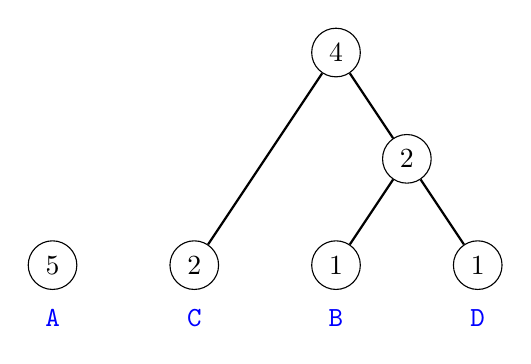
\begin{tikzpicture}[scale=0.9]
\node[draw, circle] (1) at (0,0) {$5$};
\node[draw, circle] (3) at (2,0) {$2$};
\node[draw, circle] (2) at (4,0) {$1$};
\node[draw, circle] (4) at (6,0) {$1$};
\node[draw, circle] (5) at (5,1.5) {$2$};
\node[draw, circle] (6) at (4,3) {$4$};

\node[color=blue] at (0,-0.75) {\texttt{A}};
\node[color=blue] at (2,-0.75) {\texttt{C}};
\node[color=blue] at (4,-0.75) {\texttt{B}};
\node[color=blue] at (6,-0.75) {\texttt{D}};

\path[draw,thick,-] (2) -- (5);
\path[draw,thick,-] (4) -- (5);
\path[draw,thick,-] (3) -- (6);
\path[draw,thick,-] (5) -- (6);
\end{tikzpicture}
\end{center}
Lopuksi yhdistetään kaksi viimeistä solmua:
\begin{center}
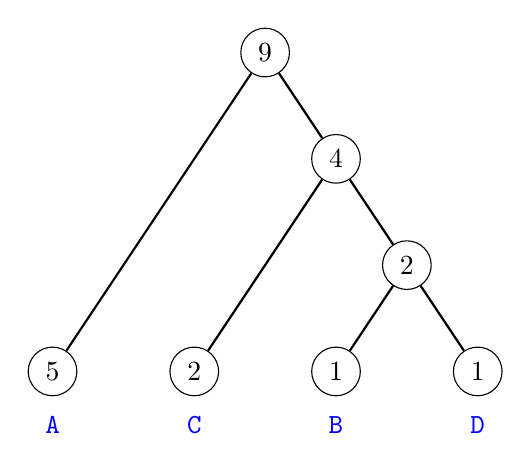
\begin{tikzpicture}[scale=0.9]
\node[draw, circle] (1) at (0,0) {$5$};
\node[draw, circle] (3) at (2,0) {$2$};
\node[draw, circle] (2) at (4,0) {$1$};
\node[draw, circle] (4) at (6,0) {$1$};
\node[draw, circle] (5) at (5,1.5) {$2$};
\node[draw, circle] (6) at (4,3) {$4$};
\node[draw, circle] (7) at (3,4.5) {$9$};

\node[color=blue] at (0,-0.75) {\texttt{A}};
\node[color=blue] at (2,-0.75) {\texttt{C}};
\node[color=blue] at (4,-0.75) {\texttt{B}};
\node[color=blue] at (6,-0.75) {\texttt{D}};

\path[draw,thick,-] (2) -- (5);
\path[draw,thick,-] (4) -- (5);
\path[draw,thick,-] (3) -- (6);
\path[draw,thick,-] (5) -- (6);
\path[draw,thick,-] (1) -- (7);
\path[draw,thick,-] (6) -- (7);
\end{tikzpicture}
\end{center}
Tuloksena olevasta puusta saadaan kutakin merkkiä vastaava
koodisana kulkemalla puun huipulta alas merkkiin asti.
Aina vasemmalle mentäessä koodisanaan tulee bitti 0
ja oikealle mentäessä koodisanaan tulee bitti 1.
Tuloksena on optimaalinen koodi:
\begin{center}
\begin{tabular}{rr}
merkki & koodisana \\
\hline
\texttt{A} & 0 \\
\texttt{B} & 110 \\
\texttt{C} & 10 \\
\texttt{D} & 111 \\
\end{tabular}
\end{center}
